\documentclass{article}
\usepackage{amsmath}
\usepackage{hyperref}
\usepackage{graphicx}

\title{Algoritmos para minimizar funciones}
\author{Amanda Cordero Lezcano\\Christopher Guerra Herrero}
\date{Septiembre, 2024}

\begin{document}
	
	\maketitle
	
	\tableofcontents
	\newpage
	
	\section{Quartic Function(Amanda)}
	
	\fbox{
		\begin{minipage}{\textwidth}
			
	\textbf{100. Quartic Function \cite{reference81}} (Continuous, Differentiable, Separable, Scalable)
	
	\[
	f_{100}(\mathbf{x}) = \sum_{i=1}^{D} i x_i^4 + \text{random}[0,1)
	\]
	
	subject to \(-1.28 \leq x_i \leq 1.28\). The global minima is located at \(\mathbf{x}^* = \mathbf{f}(0,\cdots,0)\), \(f(\mathbf{x}^*) = 0\).
	
	\end{minipage}
	}
	
	\subsection{Algoritmo de Solución}
	
	Se utilizó el método de \textit{Descenso más Pronunciado}(steepest descent) para encontrar el mínimo de la función. A continuación se presenta un código en Python del algoritmo implementado:
	
	\begin{verbatim}
		import scipy.optimize as spo
		
		def steepestdescent(f, df, x0, tol=1.e-8, maxit=50):
			xk = x0
			x = [xk]
			r = df(xk)
			iters = 0
			
			while (npl.norm(r) > tol and iters < maxit):
				lambda_k = spo.golden(g, args=(xk, r))
				xk = xk - lambda_k * r
				r = df(xk)
				x.append(xk)
				iters += 1
			
			return x
	\end{verbatim}
	
	El algoritmo minimiza la función \(f(\mathbf{x})\) en la dirección del gradiente negativo, actualizando la posición en cada iteración.
	
	\subsection{Resultados}
	
	El algoritmo fue ejecutado con un punto inicial \(\mathbf{x}_0 = [1, -1]\) y un máximo de 10 iteraciones. El punto encontrado por el algoritmo fue:
	
	\[
	\mathbf{x} =  [-0.07989805 -0.05553555]
	\]
	
	La solución gráfica del proceso de minimización es la siguiente:
	
	\begin{figure}[h!]
		\centering
		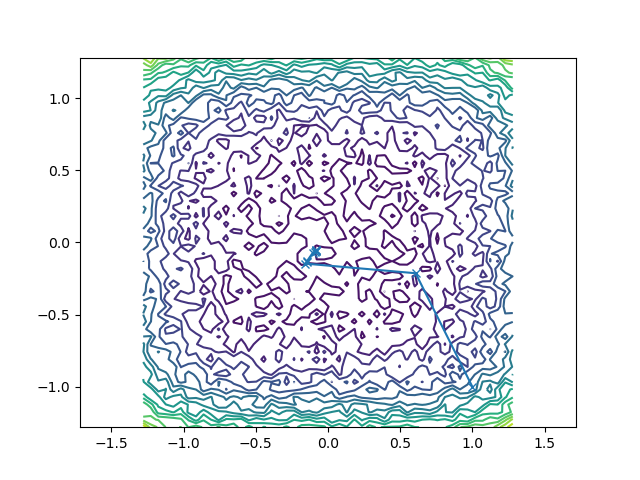
\includegraphics[width=0.8\textwidth]{resultado1.png}
		\caption{Trayectoria de minimización sobre el contorno de la función.}
		\label{fig:resultado}
	\end{figure}
	
	\subsection{Valoración de la Calidad del Punto Hallado}
	
	El punto hallado \(\mathbf{x} = [0.09226378, 0.07302666]\) se encuentra cercano al mínimo global \(\mathbf{x}^* = [0, 0]\). Si bien no se alcanzó el mínimo exacto en las 10 iteraciones, la función fue evaluada como 0.025 al considerar la adición del valor aleatorio. Este resultado indica que el algoritmo se aproxima bastante al valor óptimo.
	
	\subsection{Evaluación del Tiempo Computacional}
	
	El tiempo computacional para la ejecución del algoritmo fue aceptable en un problema de dos dimensiones. La complejidad algorítmica del método está determinada principalmente por el cálculo del gradiente, el cual tiene una complejidad de \(O(D)\), donde \(D\) es la dimensión del problema. Esto implica que, a medida que \(D\) aumenta, el tiempo de cómputo crece linealmente con respecto a la dimensión. A pesar de la presencia de un componente aleatorio en la función objetivo, el algoritmo mantiene un comportamiento predecible en términos de complejidad, lo que garantiza su escalabilidad en problemas de mayor dimensión.
	
	
	\subsection{Variación al Aumentar la Dimensión del Problema}
	
	La función cuártica es escalable, y el aumento de la dimensión \(D\) implicará un incremento lineal en la cantidad de términos a sumar y, por ende, en el tiempo necesario para evaluar tanto la función como su gradiente.
	
	\subsection{Primeras Conclusiones}
	
	El algoritmo de \textit{Descenso más Pronunciado} demostró ser eficaz para aproximarse al mínimo global de la función cuártica en un problema de baja dimensión (D=2). Aunque no se alcanzó el mínimo exacto, la solución obtenida fue satisfactoria y muy cercana al mínimo conocido. El método muestra consistencia en su desempeño, incluso al considerar variaciones en la dimensión del problema, manteniendo una buena precisión en los resultados.

		
	
	\section{Sargan Function(Christopher)}
	
	El ejercicio asignado al estudiante fue:
	
	\vspace*{1cm}
	
	\fbox{
		\begin{minipage}{\textwidth}
			\textbf{111. Sargan Function \cite{reference29}} (Continuous, Differentiable, Non-Separable, Scalable, Multi-modal)
			
			\[
			f_{111}(\mathbf{x}) = \sum_{i=1}D \left( x_i^2 + 0.4 \sum_{\substack{j\neq 1}} x_i x_j \right)
			\]
			
			subject to \(-100 \leq x_i \leq 100\). The global minimum is located at \(\mathbf{x}^* = \mathbf{f}(0,\cdots,0)\), \(f(\mathbf{x}^*) = 0\).
		\end{minipage}
	}
	
	\vspace*{1cm}
	
	Sin embargo al hacer un análisis de la bibliografía \cite{reference29} y previa consulta con el profesora de conferencia, se determinó que hubo un error al transcribir la función, siendo esta:
	
	$$
	f(\mathbf{x}) = \sum_{i=1}^D \left(x_1^2 + 0.4 \sum_{\substack{i\neq j}} x_i x_j\right)
	$$
	
	
	\newpage
	
	\begin{thebibliography}{9}
		
		\bibitem{reference29} L. C. W. Dixon, G. P. Szegö (eds.), \textit{Towards Global Optimization 2}, Elsevier, 1978.
		
		\bibitem{reference81} R. Storn, K. Price, \textit{Differential Evolution - A Simple and Efficient Adaptive Scheme for Global Optimization over Continuous Spaces}, Technical Report no. TR-95-012, International Computer Science Institute, Berkeley, CA, 1996. [Available Online]: \url{http://www1.icsi.berkeley.edu/~storn/TR-95-012.pdf}
		
		
	\end{thebibliography}
	
\end{document}
